\documentclass[a4paper,14pt]{extarticle}
\usepackage{../../tex-shared/report-layout}

\renewcommand{\mylabnumber}{5}
\renewcommand{\mylabtitle}{Исследование процессов моделирования, анализа и
                           реорганизации бизнес-процессов в методологии BPMN
                           с использованием CASE-средств}
\renewcommand{\mysubject}{Методы и средства проектирования информационных систем}
\renewcommand{\mylecturer}{Заикина Е.Н.}

\begin{document}
\begin{titlepage}
    
    \thispagestyle{empty}
    
    \begin{center}
        
        Министерство науки и Высшего образования Российской Федерации \\
        Севастопольский государственный университет \\
        Кафедра ИС
        
        \vfill

        Отчет \\
        по лабораторной работе №\mylabnumber \\
        \enquote{\mylabtitle} \\
        по дисциплине \\
        \enquote{\MakeTextUppercase{\mysubject}}

    \end{center}

    \vspace{1cm}

    \noindent\hspace{7.5cm} Выполнил студент группы ИС/б-17-2-о \\
    \null\hspace{7.5cm} Горбенко К. Н. \\
    \null\hspace{7.5cm} Проверил \\
    \null\hspace{7.5cm} \mylecturer

    \vfill

    \begin{center}
        Севастополь \\
        \the\year{}
    \end{center}

\end{titlepage}

\section{Цель работы}
Осуществить моделирование, анализ и реорганизацию бизнес-процессов с помощью
методологии BPMN. Осуществить выбор и применение инструментального средства
моделирования бизнес-процессов (BPMN-диаграммы).

\section{Задание на работу}
В соответствии с вариантом предметной области и на основании результатов
выполнения предыдущих лабораторных работ выполнить построение BPMN-диаграмм при
помощи CASE-средств: ARIS Express.

\section{Ход работы}
\begin{table}[H]
    \caption{Список задач, действующих лиц, объектов данных и показателей эффективности}
    \begin{tabular}{| p{2cm} | p{3cm} | p{5cm} | p{2.5cm} | p{2.5cm} |}
        \hline
        № задачи & Название задачи & № и список действий, составляющих решение задач & Участник, осуществляющий решение задачи & Объекты данных \\ \hline
        1 & Регистрация пользователя & Заполнение и отправка формы регистрации & Пользова- тель & БД Пользователей \\ \hline
        2 & Просмотр словарей & Выбор группы словарей, выбор словаря & Пользова- тель & БД словарей \\ \hline
        3 & Редактирова- ние словарей & Выбор группы словарей, выбор словаря, выбор перевода, редактирование & Пользова- тель & БД словарей \\\hline
        4 & Формирование упражнений & Выбор группы словарей или словаря & Пользова- тель & БД словарей \\ \hline
    \end{tabular}
\end{table}

Сформированная упрощенная диаграмма в нотации BPMN представлена на рисунке \ref{fig:simple}:
\begin{figure}[H]
    \centering
    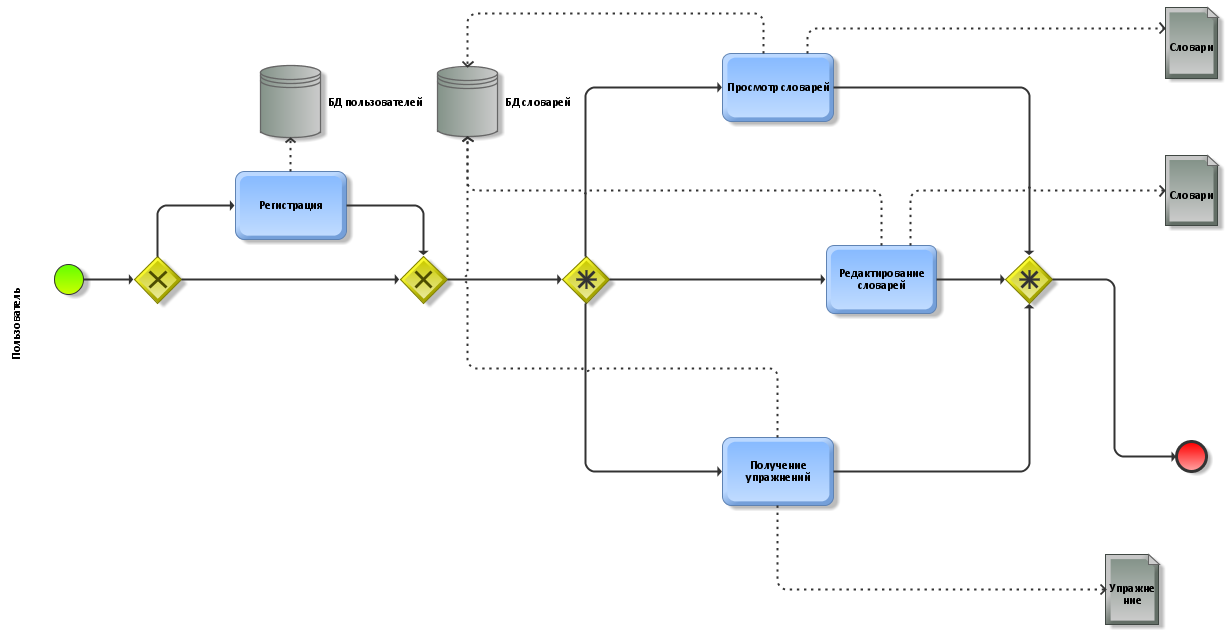
\includegraphics[width=\linewidth]{simple}
    \caption{Упрощенная диаграмма бизнес процессов в нотации BPMN}
    \label{fig:simple}
\end{figure}

Усложним модель процесса:
\begin{figure}[H]
    \centering
    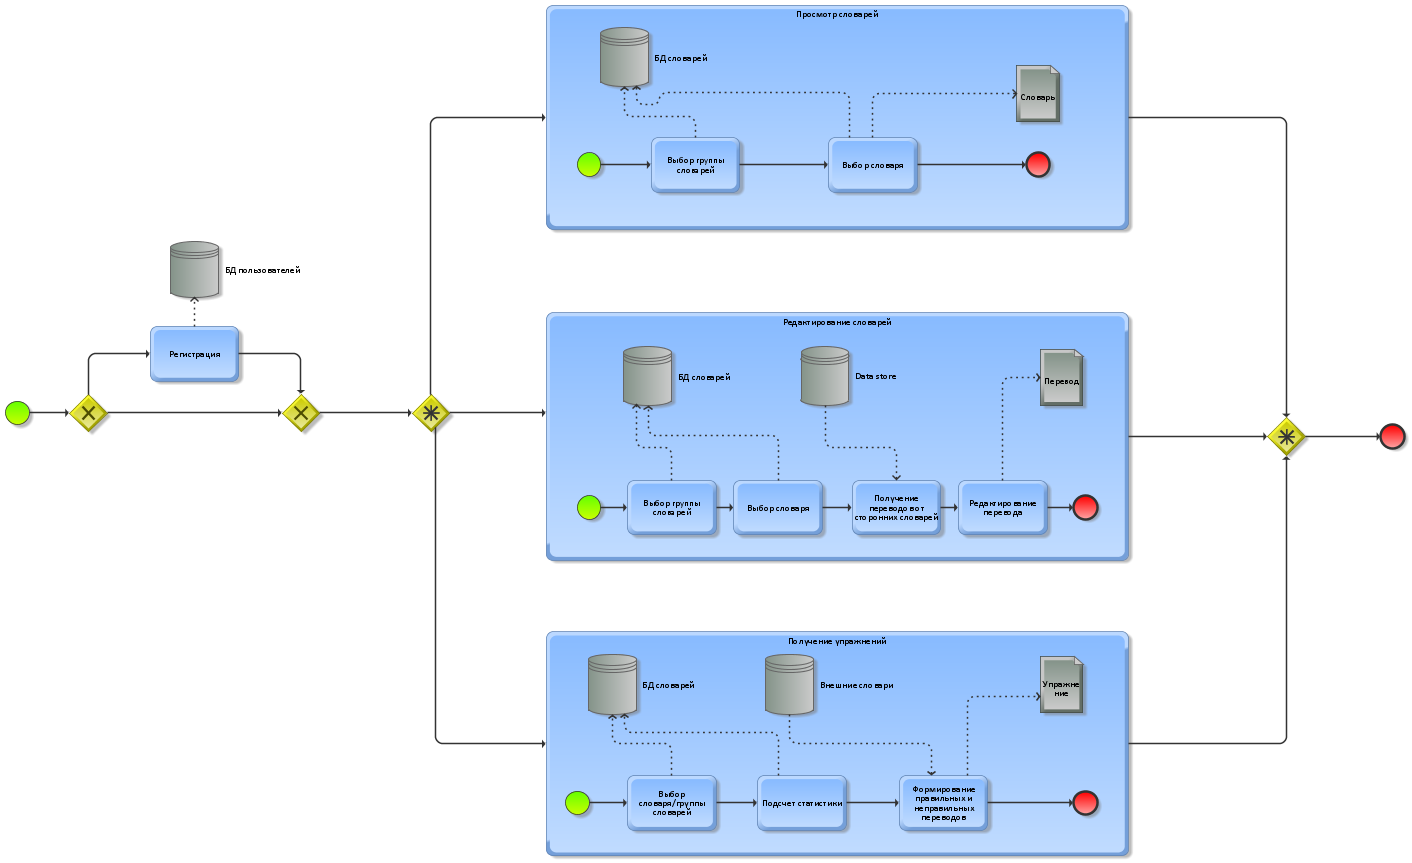
\includegraphics[width=\linewidth]{complex}
    \caption{Усложненная диаграмма бизнес процессов в нотации BPMN}
    \label{fig:complex}
\end{figure}

\section*{Выводы}
В ходе выполнения лабораторной работы было осуществлено моделирование, анализ и
реорганизация бизнес-процессов с помощью методологии BPMN. Осуществлен выбор и
применение инструментального средства моделирования бизнес-процессов
(BPMN-диаграммы).

\end{document}